\documentclass[10pt,varwidth=4cm]{standalone} 
\usepackage{tikz} 
\usepackage[labelformat=parens]{subcaption} 
\usepackage[labelformat=parens,labelsep=quad,skip=3pt]{caption} 
\usetikzlibrary{arrows,automata,calc,external} 

\tikzexternalize
 %\captionsetup[subfigure]{font={bf,small}, skip=1pt}
 \tikzset{external/system call={latex \tikzexternalcheckshellescape;
 		dvips -o "\image".eps "\image".dvi}}
 
 
 \begin{document}

 \begin{figure} 
 \tikzset{node distance=.25\textwidth}
 \begin{subfigure}[b]{\textwidth} 
 	\centering 
 	\caption{}
 		
 		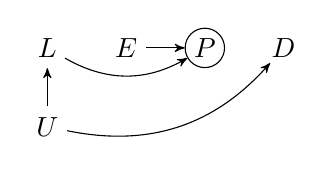
\begin{tikzpicture}[->,>=stealth',state/.style={draw,circle,minimum size=5mm, inner sep = 0pt}] 
 		\node[state,draw = none]         (L)                     {$L$};
 		\node[state,draw = none]         (U)    [below of=L]     {$U$}; 
 		\node[state,draw = none]         (E)    [right of=L]     {$E$}; 
 		\node[state,circle]              (P)    [right of=E]     {$P$}; 
 		\node[state,draw = none]         (D)    [right of=P]     {$D$}; 
 		\path (U)   edge  [bend right]   node {} (D) 
                     edge                 node {} (L) 
               (L)   edge  [bend right]   node {} (P) 
               (E)   edge                 node {} (P); 
         \end{tikzpicture} 

     \label{fig:f1a} 
 \end{subfigure} 
 \begin{subfigure}[b]{\textwidth} 
 	\centering 
 	\caption{}
  		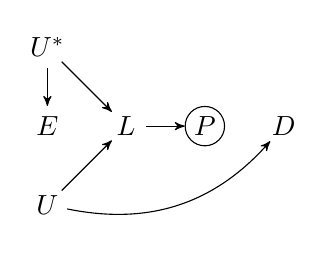
\begin{tikzpicture}[->,>=stealth',state/.style={draw,circle,minimum size=5mm, inner sep = 0pt}] 
 		\node[state,draw = none]         (Us)                    {$U^{*}$}; 
 		\node[state,draw = none]         (E)    [below of=Us]    {$E$}; 
 		\node[state,draw = none]         (U)    [below of=E]     {$U$}; 
 		\node[state,draw = none]         (L)    [right of=E]     {$L$}; 
 		\node[state,circle]              (P)    [right of=L]     {$P$}; 
 		\node[state,draw = none]         (D)    [right of=P]     {$D$}; 
 		\path (Us)  edge                 node {} (E) 
 		            edge                 node {} (L) 
 		      (U)   edge  [bend right]   node {} (D) 
 		            edge                 node {} (L) 
 		      (L)   edge                 node {} (P); 
 		\end{tikzpicture} 
 	\label{fig:f1b} 
 \end{subfigure} 
 \begin{subfigure}[b]{\textwidth}
 	\centering 
 	\caption{}
  		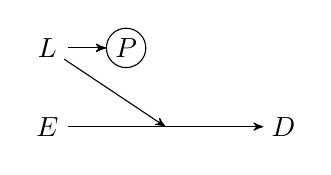
\begin{tikzpicture}[->,>=stealth',state/.style={draw,circle,minimum size=5mm, inner sep = 0pt}] 
 		\node[state,draw = none]         (L)                     {$L$};
 		\node[state,draw = none]         (E)    [below of=L]     {$E$}; 
 		\node[state,circle]              (P)    [right of=L]     {$P$}; 
 		\node[]                          (x1)   [right of=P]     {}; 
 		\node[]                          (x2)   [right of=x1]    {}; 
 		\node[state,draw = none]         (D)    [below of=x2]    {$D$}; 
 		 
 		\path (L)   edge                 node {} (P) 
 		            edge                 node {} (P) 
 		      (E)   edge                 node {} (D); 
 		       
 		\draw (L)                    --  node {} ($(E)!0.5!(D)$); 
 		\end{tikzpicture} 
 	\label{fig:f1c} 
 \end{subfigure} 
  
 %\begin{tikzpicture}[->,>=stealth',shorten >=1pt,auto,node distance=2.5cm,semithick] 
 % 
 %\node[state,draw = none]         (U*)              {$U^{*}$}; 
 %\node[state,draw = none]         (M) [below of=U*] {$M$}; 
 %\node[state,draw = none]         (E) [right of=M]  {$E$}; 
 %\node[state,circle]              (C) [right of=E]  {$C$}; 
 %\node[state,draw = none]         (O) [right of=C]  {$O$}; 
 %\node[state,draw = none]         (U) [below of=M]  {$U$}; 
  
 %\path (U*) edge              node {} (E) 
 %edge              node {} (C) 
 %(M)  edge [bend right] node {} (C) 
 %(U)  edge              node {} (M) 
 %edge [bend right] node {} (O); 
 %\end{tikzpicture} 
  
 \end{figure} 
 \end{document} 
  
